%%%%%%%%%%%%%%%%%%%%%%%%%%%%%%%%%%%%%%%%%%%%%%%%%%%%%%%%%%%%%%%%%%%%%%%
%
%   Presentation of Beamer UNL Theme
%   Beamer Presentation by Chris Bourke
%
%%%%%%%%%%%%%%%%%%%%%%%%%%%%%%%%%%%%%%%%%%%%%%%%%%%%%%%%%%%%%%%%%%%%%%%

\documentclass{beamer}

\usetheme[hideothersubsections]{UNLTheme}
\usepackage[postscript]{ucs}
\usepackage[utf8x]{inputenc}
\usepackage{amsmath}
\usepackage{amssymb}
\usepackage{amsthm}
\usepackage{mathtools}
\title{Performance Modeling and
Design of Computer Systems- Ch 13 \\
M/M/1 and PASTA}
\author{Debobroto Das Robin} %
\institute{Kent State University}
\date{Spring 2020}




\begin{document}

%{% open a Local TeX Group
%\setbeamertemplate{sidebar}{}
\begin{frame}
        \titlepage
        \begin{center}
    \href{mailto:drobin@kent.edu}{\color{blue}{\texttt{drobin@kent.edu}}}
        \end{center}
\end{frame}

\begin{frame}
\frametitle{Overview} % Table of contents slide, comment this block out to remove it
\tableofcontents % Throughout your presentation, if you choose to use \section{} and \subsection{} commands, these will automatically be printed on this slide as an overview of your presentation
\end{frame}



\section {The M/M/1 Queue }



\begin{frame} 
\frametitle{The M/M/1 Queue-1 }
\framesubtitle{\textbf{\textit{}}}
\begin{itemize}
\item  \textbf{M/M/1 Queue:}simplest queueing model consisting single server 
\item Service times are i.i.d. Exponential random variables with mean $1\mu$,  
\item Jobs arrive according to a Poisson process with rate $\lambda$. 
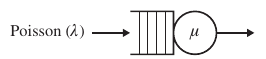
\includegraphics[scale=.7]{images/mm1queu.jpeg}
\item \textbf{M/M/p/q:} 4 slot Kendall Notation. \textbf{1st M}: arrival process-- ``memoryless''. \textbf{2nd M:} distribution of the service -- ``memoryless'' -- ``exponential'' \textbf{3rd ``p'':}  number of servers in the system . \textbf{4th ``q'':}upper bound on the capacity of the system in terms of the total space available to hold jobs. \textbf{\textit{absence of a fourth field
indicates that the queue is unbounded and that the scheduling policy is FCFS}}

\end{itemize}

\end{frame}

\begin{frame} 
\frametitle{The M/M/1 Queue-2 }
\framesubtitle{\textbf{\textit{}}}
\begin{itemize}
\item  \textbf{Number of customers} in an M/M/1 system forms a continuous-time Markov chain
(CTMC) where the \textbf{state} of the system corresponds to the \textbf{number of customers} in the
system.
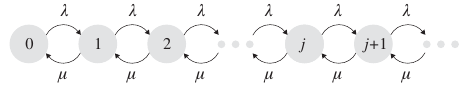
\includegraphics[scale=.7]{images/mm1CTMC.jpeg}
\item A.K.A. \textbf{birth-death process}, with $\lambda$ -- ``births'' and the $\mu$ -- ``deaths''
\item Rate of transitions leaving state $i$ to go to state $i+1 = \pi_i\lambda$ 
\item Solution of Balance Equation: $\pi_i = (\frac{\lambda}{\mu})^i \pi_0$ (page 237 for details)
\end{itemize}

\end{frame}

\begin{frame} 
\frametitle{The M/M/1 Queue-3 }
\framesubtitle{\textbf{\textit{Important Metrics : For derivation look at section 13.1}}}
\begin{itemize}
\item  \textbf{ server utilization} = $\rho = \frac{\lambda}{\mu} $
\item  $\rho < 1$  must be met if the system is to be stable (number of jobs not grows without bound). For this
condition to be true, we must ${\lambda}<{\mu}$
\item mean number of customers in the system = $E[N] = \frac{\rho}{1-\rho}$
\item variance of the number of customers = $Var(N) = \frac{\rho}{{(1-\rho)}^2}$

\end{itemize}

\end{frame}

\section{M/M/1 Queue Example}
\begin{frame} 
\frametitle{M/M/1 Queue Example}
\framesubtitle{\textbf{\textit{ Increasing Arrival and Service Rates Proportionally}}}
\begin{itemize}
\item  \textbf{Q.} Given an M/M/1 system (with $\lambda < \mu$), if arrival rate $\lambda$ \& service rate $\mu$ are both increased $k$ times, What the impact on system performance?
\item \textbf{Ans:} $$ \lambda_{new} = k\lambda \:, \: \mu_{new} = k\mu $$
\item Utilization rate = $\rho_{new} = \frac{\lambda_{new}}{\mu_{new}}= \rho_{old}$
\item Expected number of jobs $E[N_{new}] = \frac{\rho{new}}{1-\rho{new}} \frac{\rho{old}}{1-\rho{old}} = E[N_{old}]$

\item Response time = $E[T_{new}] = \frac{1}{\mu_{new}-\lambda{new}} = \frac{1}{k(\mu-\lambda)}  = \frac{1}{k} E[T_{old}]$
\end{itemize}
\end{frame}

\section{PASTA }
\begin{frame} 
\frametitle{PASTA }
\framesubtitle{\textbf{\textit{ Poisson Arrivals See Time Averages)}}}
\begin{itemize}
\item Precondition: Arrival process have to be Poisson
\item  $\pi_n= p_n$ = limiting probability that there are n jobs in the system 
\item $a_n$= limiting probability that an arrival
sees n jobs in the system 
\item $d_n$= limiting probability that a departure leaves behind n jobs in the system when it departs 
\item \textbf{PASTA}:  If the arrival process to the system is a Poisson process, then $a_n = p_n$
\item Application:  If we are simulating a Poisson arrival process
to some system and would like to know the mean number of jobs in the system. 

\end{itemize}
\end{frame}
\end{document}